\section{Introduction}

Clearly OpenMP\cite{Ope00}\cite{Ope02} has become the leading industry
standard for parallel programming on shared memory and distributed
shared memory multiprocessors. Although there are different
hardware architectures to support the programming model, the
implementation of an OpenMP programming language usually can be
separated into two parts: compilation process and runtime support,
shown in Figure \ref{fig:runtime}.
In this figure, the language-dependent frontends will translate user
source code to an \emph{intermediate representation (IR)}, to be
processed by an optimizing compiler into a resulting \emph{node
program}, which interacts with a \emph{runtime} environment that
starts and controls the multi-threaded execution.

\begin{figure}[!h]
  \begin{center}
    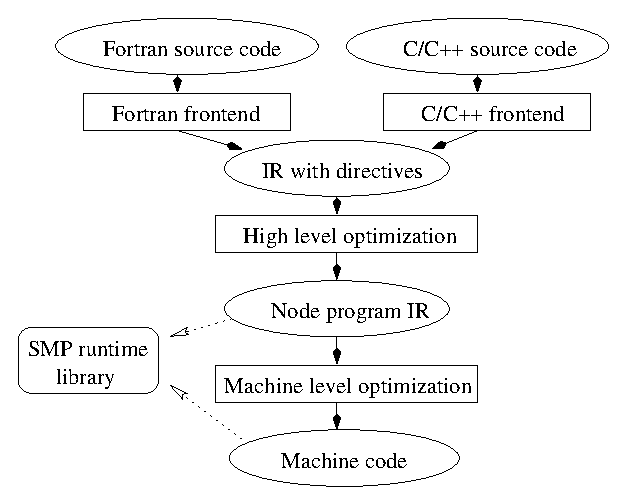
\includegraphics[angle=0, width=0.65\textwidth]{runtime.eps}
    \caption{\footnotesize compilation structure}
    \label{fig:runtime}
  \end{center}
\end{figure}

%Jointly defined by a group of major computer hardware
%and software vendors, OpenMP is a portable, scalable model that gives
%shared-memory parallel programmers a simple and flexible interface for
%developing parallel applications for platforms ranging from the
%desktop to the supercomputer.

%Figure \ref{fig:runtime} shows the general compilation and runtime
%structure for parallelizing compilers. 


%This is a common strategy used by many previous works $need more$
%\cite{lcpc97}.

There are already papers introducing the compilation part of this
structure \cite{Wom03}, yet little discussion has been dedicated to
the runtime environment itself. In fact, as the OpenMP standard
continues evolving, there are still many open issues in this area,
such as the mechanisms required to support nested parallelism,
threadprivate etc.

In this paper, we will focus our attention on the runtime environment
implementation. The runtime system we have developed is based on the
pthreads library available on most major operating systems, including
Linux, Mac OS and AIX\copyright.

We try to avoid the controversial parts of the OpenMP runtime
environment by concentrating mainly on structures and algorithms used
to implement OpenMP \emph{workshares}, the well-understood concept yet
the most fundamental one in parallel programming. We will also discuss
the performance considerations when we use standard benchmarks to 
test our implementation.

%General speaking, the amount of thread local storage can not be
%determined statically. Because it is not clear at compile time that how
%many threads will be created to execute the OpenMP program. The total
%amount of memory used is better to be decided at run time dynamically.



